\subsection{Statistische Analyse von Höhendaten}
\usetikzlibrary{decorations.pathreplacing}
Ausserhalb der gewöhnlichen statistischen Analyse, die wir
hier als bekannt voraussetzen, führen wir hier weitere Werkzeuge
ein, die sich spezial für die Analyse rauer Oberflächen bzw. 
Gitterstrukturen als nützlich erweisen\cite{gwyddion}. Zunächst
gehen wir davon aus, dass uns die Mikroskopiedaten als 
$N \times M$ Vektorfeld vorliegen (N Zeilen und M Spalten der
Matrix der Bilddaten, ). Die tatsächliche Fläche der Daten
nennen wir nun $L_x \times L_y$, wobei 
wir ObdA nehmen nun annehmen, dass die Abstände
zwischen den Datenpunkten $\Delta$ betrage 
(siehe Abbildung~\ref{fig:stat1}). 

\begin{figure}
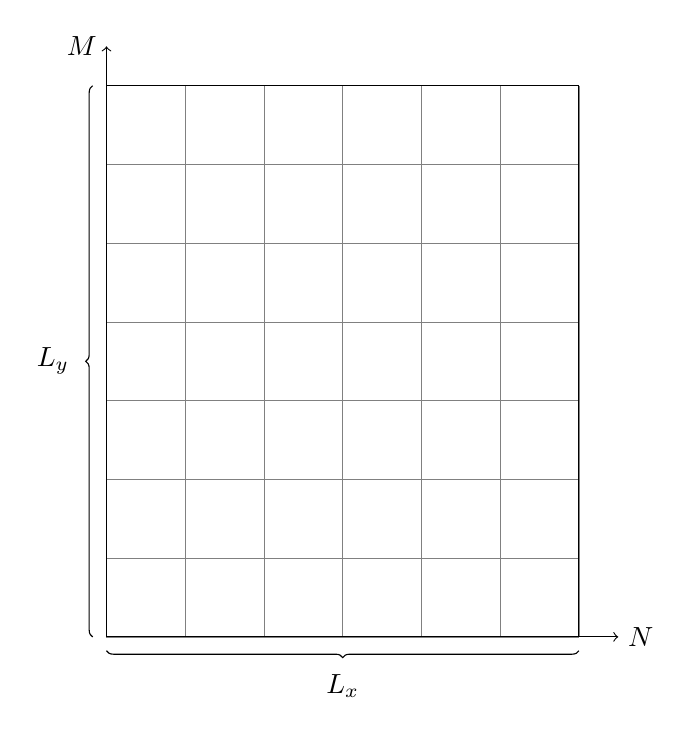
\begin{tikzpicture}
\draw[step=1cm,gray,very thin] (-1,-1) grid (5,6);
\draw  (-1,-1) -- (5,-1) -- (5,6) -- (-1,6) -- (-1,-1);
\draw [<->] (-1,6.5) node [left]{$M$} -- (-1,-1) 
-- (5.5,-1) node [right] {$N$};
\draw [decoration={brace,mirror,raise=5pt},decorate]
(-1,-1) --  node[below=10pt]{$L_x$}(5,-1); 

\draw [decoration={brace,raise=5pt},decorate]
(-1,-1) --  node[left=10pt]{$L_y$}(-1,6); 

\end{tikzpicture}
\caption{Das Vektorfeld der Mikroskopiedaten besteht aus 
$N \times M$ Höhendaten aus $\mathbb{R}$, wobei die tatsächliche 
Fläche $L_x \times L_y$ beträgt.}
\label{fig:stat1}
\end{figure}
Wir betrachten nun 
die statistischen Eigenschaften der Zufallsvariablen $\xi(x,y)$. 
Die Wahrscheinlichkeitsdichte $\rho(x,y,z)$ für eine 
bestimmte Höhe $z$ ergibt sich numerisch
durch die Extrapolation der einzelnen Datenpunkte mit der Normierung:
\begin{equation*}
\int \rho(x,y,z) dx dy dz = 1
\end{equation*}
\subsubsection{Fourier Transformationen und Leistungsspektrum}
Sei nun ganz allgemein die Fouriertransformation eingeführt:
\begin{align}
f(x) = \int_{-\infty}^{\infty} F(k)\exp(2\pi kx)dk\\
F(x) = \mathcal{F}_x\left [f(x)\right ](k) =
\int_{-\infty}^{\infty} f(k)\exp(-2\pi kx)dx
\end{align}
Mit den Eigenschaften:
\begin{align}
\mathcal{F}\left [a f(x) + b g(x)\right ]
    = a F(k) + b G(k)\\ 
   % \mbox{ (Linearität) }\\

\end{align}
\begin{align}
\mathcal{F}\left [f(x) * g(x)\right ](k)
    = \mathcal{F}\left [f(x)\right ]\mathcal{F}\left [g(x)\right ]\\
    %\! \mbox{ (Faltungseigenschaft, wobei $f*g$ die Faltung ist) }\\
\mathcal{F}_k\left [\left | F(k) \right |^2\right ](x)
   =  \int_{-\infty}^{\infty}\bar{f}(\tau)f(\tau + x) d\tau 
   %\mbox{ Wiener-Khinchin Theorem }
\end{align}
